%********************************************************************
% Appendix
%*******************************************************

\addcontentsline{toc}{part}{Anhang}
\markright{Anhang}


\chapter{Beantwortung der Versuchsfragen}
  
\begin{enumerate}
		\item \textbf{Welche Rahmen dienen der TEI-Vergabe, und welcher TEI-Wert wird
		dem Telefon von der Vermittlung zugewiesen?}
		\newline
		F�r die TEI-Vergabe dienen die Rahmen der Nachrichten ``Identity Request'' und
		''Identity Assigned''. Es handelt sich um U-Frames. Dem Telefon (Telefon 1 mit
		MSN 100) wird der TEI-Wert 64 von der Vermittlungsstelle zugewiesen.
		\newline
		\textit{siehe Anhang B: Frame 56 und 57}
		\item \textbf{Wann ist der Aufbau der Schicht 2 abgeschlossen?}
		\newline
		Nach Senden der SABME-Nachricht, welche die VSt mit einer UA-Nachricht
		beantwort, ist Schicht 2 aufgebaut.
		\newline
		\textit{siehe Anhang B: Frame 338 und 339}
		\item \textbf{Welchen ISDN-Dienst fordert das Telefon von der
		Vermittlungsstelle an, welche �bertragungskapazit�t ben�tigt dieser Dienst?}
		\newline
		Das Telefon fordert von der VSt den Dienst der Sprach�bertragung an. Diese
		Information ist der SETUP-Nachricht zu entnehmen, ebenso wie die
		�bertragunskapazit�t:
		\newline
		Information transfer capability: Speech (0x00)
		\newline
		Information transfer rate: 64 kbit/s (0x10)
		\newline
		\textit{siehe Anhang B: Frame 340}
		\item \textbf{Welche Kodierung des Sprachkanals wird gew�hlt?}
		\newline
		Auch die Kodierung ist der SETUP-Nachricht zu entnehmen.
		\newline
		Coding standard: ITU-T standardized coding (0x00)
		\newline
		\textit{siehe Anhang B: Frame 340}
		\item \textbf{Welche MSN-Nummer wird in welchem Rahmen �bertragen?}
		\newline
		Die MSN des anrufenden Teilnehmers wird mit der SETUP-Nachrijct �bertragen:
		Calling Party Number. Die Zielrufnummer wird bei Einzelwahl in den
		Informationsnachrichten �bertragen.
		\newline
		\textit{siehe Anhang B: Frame 344, 346, 348}
		\newline
		Bei einer Blockwahl wird die MSN der Zielrufnummer in der SETUP-Nachricht
		�bermittelt: Called Party Number.
		\newline
		\textit{siehe Anhang B: Frame 366}
		\item \textbf{Wann ist der gesicherte Aufbau der Schicht 3 abgeschlossen?}
		\newline
		Der gesicherte Aufbau der Schicht 3 ist nach Erhalt der CONNECTION ACHNOWLEDGE
		abgeschlossen.
		\newline
		\textit{siehe Anhang B: Frame xxx}
		\item \textbf{Welchen B-Kanal weist die Vermittlung der Verbindung zu?}
		\newline
		Der Verbindung wird der B-Kanal 1 zugewiesen (B1 Channel)
		\newline
		\textit{siehe Anhang B: Frame 350}
		\item \textbf{Wo wird die gerufene Telefonnummer �bermittelt?}
		\newline
		Diese Frage wurde bereits unter 5. beantwortet.
		\item \textbf{Mit welchem Rahmen best�tigt die Vermittlung die Vollst�ndigkeit
		der Rufnummer und beginnt den angeforderten Teilnehmer anzuw�hlen?}
		\newline
		Die Vollst�ndigkeit wird durch das Senden der CALL PROCEEDING Nachricht
		best�tigt.
		\newline
		\textit{siehe Anhang B: Frame 350}
		\item \textbf{Mit welchem Rahmen signalisiert die Vermittlung, dass der
		gerufene Teilnehmeranschluss ein Endger�t besitzt, das den Sprachdienst
		erf�llen kann und ein Rufsignal aussendet?}
		\newline
		Dies geschieht mit der ALERTING-Nachricht von der VSt.
		\newline
		\textit{siehe Anhang B: Frame 352}
		\item \textbf{Wann sind die Schichten 3 und 2 jeweils wieder vollst�ndig
		abgebaut?}
		\newline
		Schicht 3 ist mit Senden des RELEASE COMPLETE abgebaut. Nach DISC ist auch
		Schicht 2 wieder abgebaut.
		\newline
		\textit{siehe Anhang B: Frame 360 und 362}
		\item \textbf{Bei ISDN gibt es die M�glichkeit, bei einem abgehenden Ruf die
		Zielrufnummer vor oder nach dem Abheben des H�rers einzugeben. Wodurch
		unterscheidet sich die Signalisierung auf Schicht 3 (SETUP- und
		INFO-Nachricht) der Teilnehmerschnittstelle in diesen beiden F�llen? F�hren
		Sie dazu einen erneuten Call mit aufgelegtem H�rer (= Blockwahl) durch.}
		\newline
		Beim normalen Anruf, d.h. bei Einzelwahl ist die Zielrufnummer zum Zeitpunkt
		der SETUP-Nachricht noch nicht bekannt. Die Ziffern der Rufnummer werden im
		Anschluss einzeln in INFO-Nachrichten zur VSt gesendet bis diese vollst�ndig
		ist (siehe Aufgabe 5). Bei Blockwahl hingegen ist die Zielrufnummer in der
		SETUP-Nachricht im Nachrichtenelement ``Called Party Number'' enthalten.
		\newline
		\textit{siehe Anhang B: Frame 366}
\end{enumerate}

\chapter{Ausz�ge des Protokollmitschnitts}
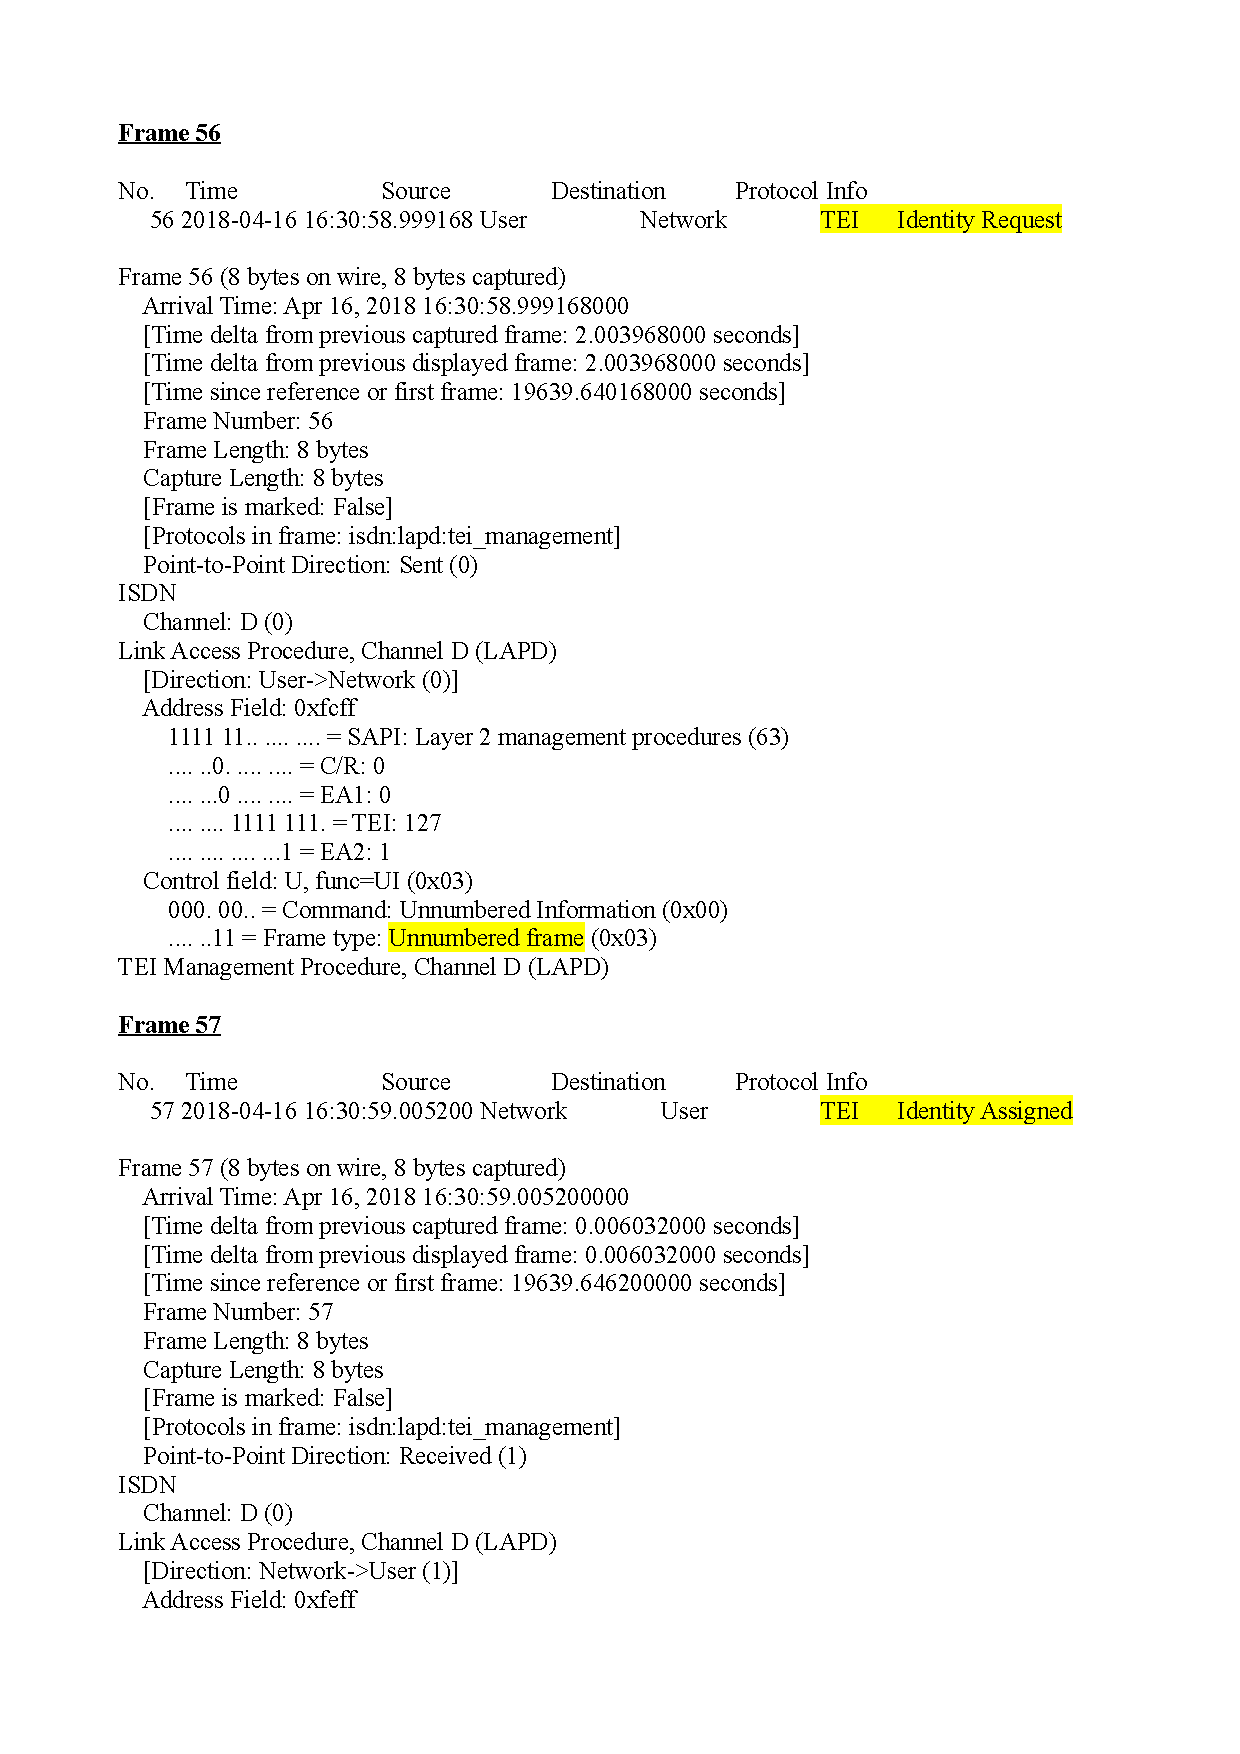
\includepdf[pages={1-12}]{Chapters/Auszuege.pdf}

